% !TEX TS-program = pdflatex
% !TEX encoding = UTF-8 Unicode
% !TEX root = ../main.tex
% !TEX spellcheck = en-US
% ****************************************************************************************
% File: methods.tex
% Author: Jakob Spindler
% Date: 2024-10-16
% ****************************************************************************************
\chapter{Methods}
\label{chapter:methods}

The PLECS model of the converter includes the following:
\begin{itemize}
    \item a PID controlled duty cycle
    \item a noise source for the input voltage
    \item a variable load
\end{itemize}

all of which can be selected to be active or inactive as can be seen in \autoref{fig:PLECS_model} and \autoref{fig:PLECS_subsystems}.

\begin{figure}[htbp]
    \centering
    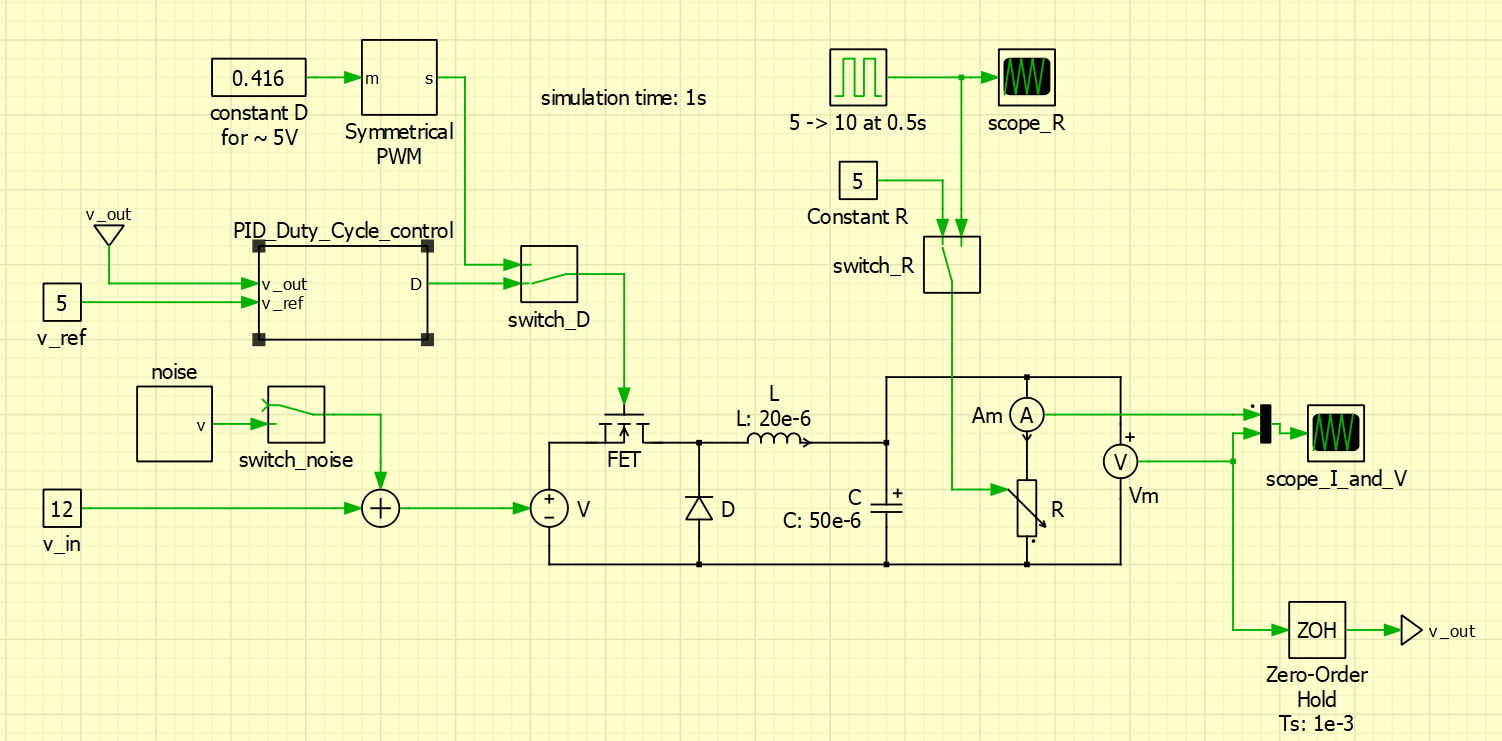
\includegraphics[width=0.95\textwidth]{img/PLECS_model_full_view.png}
    \caption{PLECS model of the Buck-Converter}
    \label{fig:PLECS_model}
\end{figure}

\begin{figure}[htbp]
    \centering
    \begin{subfigure}[b]{0.55\textwidth}
        \centering
        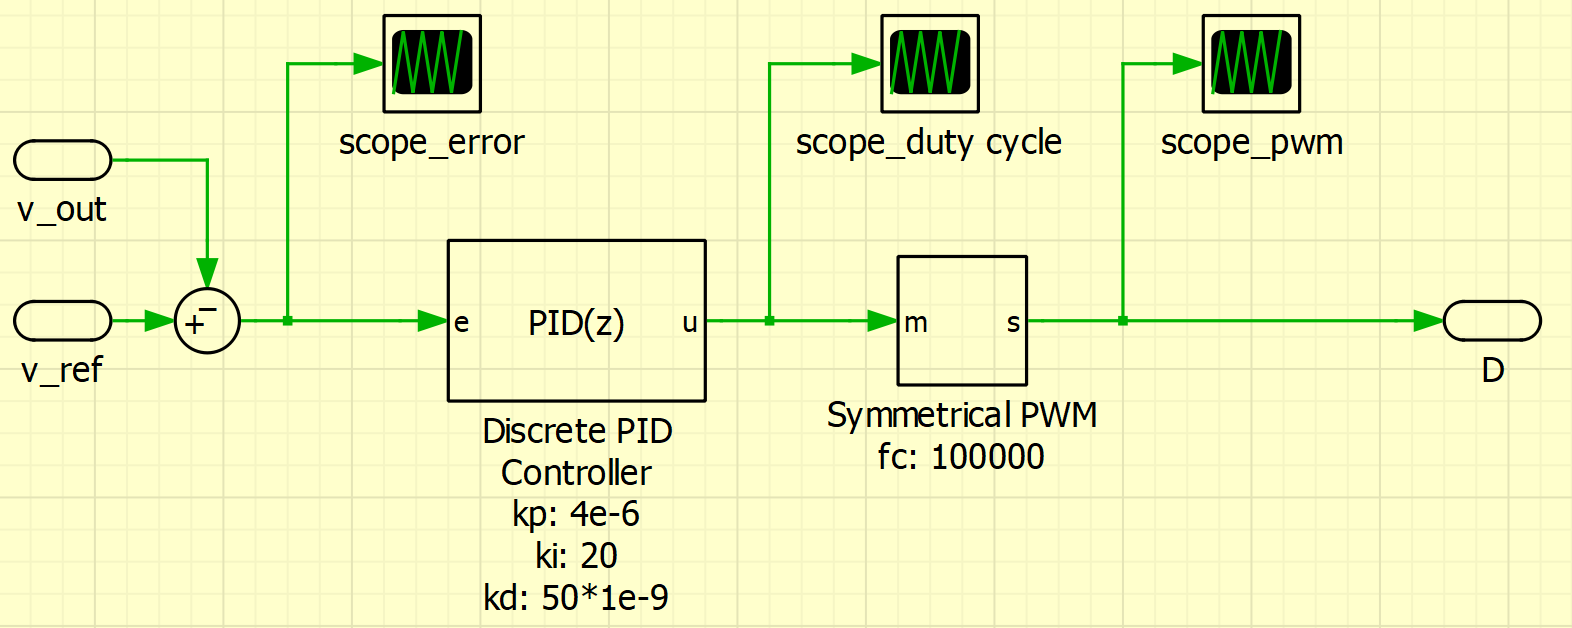
\includegraphics[width=\textwidth]{img/PLECS_PID_Duty_Cycle_control.png}
        \caption{PLECS model of the PID\_Duty\_Cycle\_control subsystem}
        \label{fig:PLECS_PID}
    \end{subfigure}
    \hfill
    \begin{subfigure}[b]{0.40\textwidth}
        \centering
        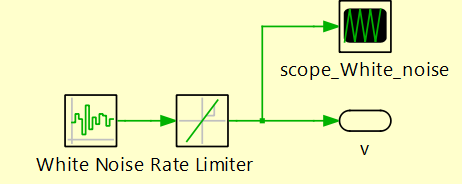
\includegraphics[width=\textwidth]{img/PLECS_noise.png}
        \caption{PLECS model of the noise subsystem}
        \label{fig:PLECS_noise}
    \end{subfigure}
    \caption{PLECS model subsystems}
    \label{fig:PLECS_subsystems}
\end{figure}

\begin{figure}[htbp]
    \centering
    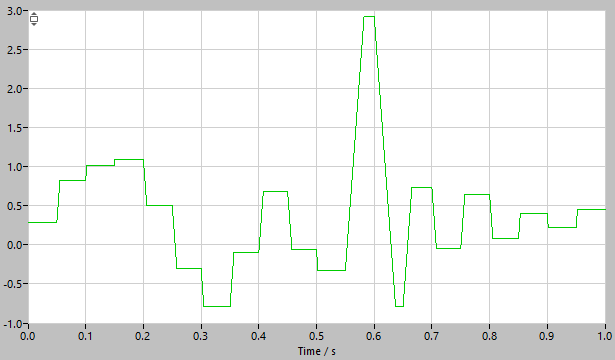
\includegraphics[width=0.8\textwidth]{img/noise.png}
    \caption{White noise with a standard deviation of \qty{1}{\volt} and a sample time of \qty{50}{\milli\second}}
    \label{fig:noise}
\end{figure}

The control of the converter was tested under the following conditions and compared to the behaviour of the converter with a fixed duty cycle:
\begin{itemize}
    \item noise on the input voltage (white noise with a standard deviation of \qty{1}{\volt} and a sample time of \qty{50}{\milli\second} as seen in \autoref{fig:noise})
    \item a load step from \qty{5}{\ohm} to \qty{10}{\ohm} at \qty{0.5}{\second}
    \item startup behaviour
\end{itemize}


% EOF